% Knowledge as Dynamics.
% Compile: tectonic main.tex   (figures in ./figures/)
\documentclass[11pt]{article}

\usepackage[margin=1in]{geometry}
\usepackage{amsmath,amssymb}
\usepackage{graphicx}
\usepackage{tikz}
\usepackage{microtype}
\usepackage{caption}
\usepackage{xurl}
\usepackage{etoolbox}
\usepackage{parskip}
\usepackage{titlesec}
\usepackage[round]{natbib}
\usepackage[colorlinks=true,linkcolor=blue,citecolor=blue,urlcolor=blue]{hyperref}

\captionsetup{font=small,labelfont=bf}

% Air around headings.
\titlespacing*{\section}{0pt}{2.2em plus .4em}{1.0em}
\titlespacing*{\subsection}{0pt}{1.6em}{0.8em}

% Plain-terms passages for the lay reader.
\newenvironment{plainterms}{\par\medskip\noindent\itshape In plain terms.\ }{\par\medskip}

% Pull the title block up so the hero figure fits on the first page.
\makeatletter
\patchcmd{\@maketitle}{\newpage\null\vskip 2em}{\newpage\vspace*{-2.6em}}{}{%
  \GenericError{}{maketitle patch failed}{}{}}
\makeatother

\newcommand{\enc}{E}
\newcommand{\dec}{D}
\newcommand{\Vfield}{V}

\title{Knowledge as Dynamics}

\author{%
Elias Helou\\
Veso AI\\
\texttt{elias.helou@veso.ai}
\and
Ivan Nemytchenko\\
Independent researcher\\
\texttt{nemytchenko@gmail.com}
}

\date{v1.4, July 15, 2026\\[0.5em]

\begin{tikzpicture}[x=0.013cm,y=0.013cm]
\fill[black] (63.02,0.00) -- (30.75,0.00) -- (40.08,27.92) -- (22.39,19.09) -- (0.82,40.66) -- (38.35,60.06) -- (13.87,80.94) -- (25.28,109.22) -- (58.15,81.99) -- (68.49,112.91) -- (98.99,112.91) -- (90.79,87.16) -- (106.09,95.07) -- (128.92,72.25) -- (92.09,53.87) -- (116.53,33.62) -- (104.46,3.69) -- (72.80,30.68) -- (63.02,0.00) -- cycle;
\end{tikzpicture}}

\begin{document}
\maketitle
\thispagestyle{empty}
\enlargethispage{2\baselineskip}
\vspace{-1.2em}

\section{Introduction}

A neural network's knowledge can be copied without a single training example. A trained autoencoder moves every point of its latent space by $\Vfield(z) = \enc(\dec(z)) - z$. Training carves attractors into this field. A fresh network trained only to match $\Vfield$, with no data and no weights, inherits the teacher's basins of attraction (Figure~\ref{fig:hero}). Transfer, merging, and preservation of knowledge then become operations on vector fields, with fidelity that can be measured and priced before training.

Think of the latent space as a hilly landscape. A marble dropped anywhere rolls into one of a few valleys; the valleys are the learned concepts, and the terrain is the knowledge. We copy the terrain the way a surveyor would: query the slope at many points and rebuild the landscape from the answers.

\begin{center}
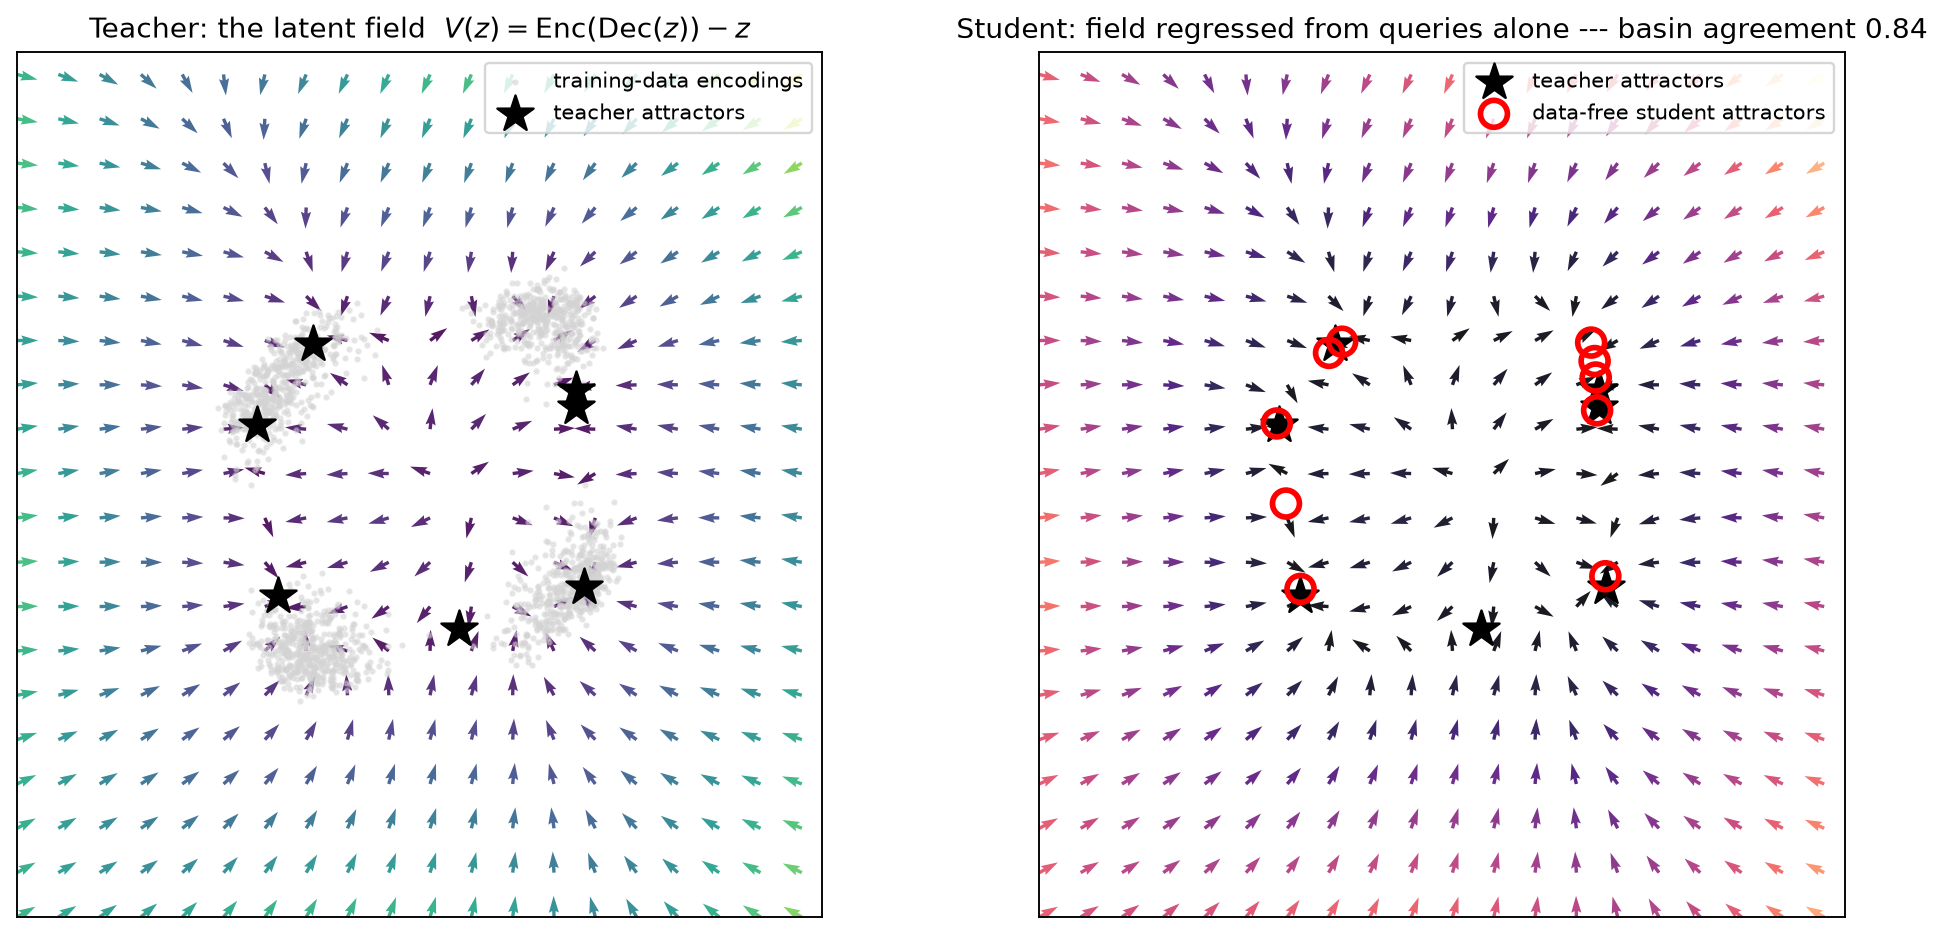
\includegraphics[width=0.92\linewidth]{figures/hero.png}
\captionof{figure}{\textbf{The core effect.} Left: the teacher network's terrain. Each arrow shows which way a point moves when the network re-processes it; black stars mark the valleys (attractors) that training carved. Right: a new network rebuilt from slope queries alone, with no data and no weights. Its valleys (red circles) land on the teacher's stars, and $84\%$ of test points reach the same valley in both networks.}
\label{fig:hero}
\end{center}

\paragraph{Thesis.} A network's learned structure lives in its latent vector field and transmits through it. The quality, reliability, and generational fate of that transmission are governed by one teacher-only measurement: the geometry of the teacher's basin boundaries, read from the flip-rate curve $f(\varepsilon)$ and its uncertainty exponent $\alpha$. This measurement ordered transfer quality at Spearman $+1.0$ in every system tested: exact mathematics, a physical flow, and learned networks.

The paper fixes the object and six procedures, then presents twelve findings in four groups: the field suffices and static channels do not; mean error is the wrong observable; fields compose and inherit, with loss and selection located in the carrier; the $\alpha$ diagnostic holds at ground truth. The conclusion states the next stage: a knowledge benchmark built on these instruments. Every number has a released JSON run record, and all experiments ran in MLX on one Apple laptop, the full suite in under an hour.

\section{The Object and the Procedures}

The object of study is the dynamical system an autoencoder induces on its own latent space. The composite map $f(z) = \enc(\dec(z))$ defines $z_{t+1} = f(z_t)$; its displacement field is $\Vfield(z) = f(z) - z$; attracting fixed points and their basins summarize what the network learned \citep{fumero2025}. Standard distillation instead matches static snapshots of one forward pass: outputs \citep{hinton2015}, features \citep{romero2015fitnets}, relations among embeddings \citep{park2019rkd,tung2019similarity,tian2020crd}, input--output Jacobians \citep{srinivas2018jacobian}, or fixed latent geometry \citep{medal2026,latentmanifolds2026}. Six procedures turn the field itself into a channel.

\paragraph{P1: Field distillation (data-free).} Regress a fresh student's field onto the teacher's at sampled latent points,
\begin{equation}
  \mathcal{L} \;=\; \mathbb{E}_{z \sim p(z)} \big\| \Vfield_s(z) - \Vfield_t(z) \big\|^2 .
\end{equation}
No training data and no weights are used; the teacher is queried only through its latent self-map. A small reconstruction anchor ($0.2$ weight, $5\%$ of data) is added only when data-space behavior is required.

\paragraph{P2: Cross-model comparison.} Fit an affine map $A(z) = zW + b$ by least squares between student and teacher encodings. Compare fields in teacher coordinates. Grant every method the better of \{identity, fitted affine\}.

\paragraph{P3: Evaluation.} Field NMSE and mean cosine over probes where $\|\Vfield_t\|$ exceeds its 10th percentile. Basin agreement: iterate probes 300--1{,}000 steps and score the fraction of endpoints that match the reference within tolerance $\varepsilon$. Always report the self-agreement ceiling (the source against itself under small probe perturbations) and the convergence fraction. Attractor recovery: symmetric Chamfer distance between attractor sets. Held-out reconstruction. Falsification criteria are fixed before each run.

\paragraph{P4: Union frames (composition).} A common frame holds teacher $A$'s chart natively. Teacher $B$'s chart enters through an affine conjugacy $T$. The union field is a gated superposition with a nearest-centroid gate. $T$ must be isometric: a pure translation into empty frame territory (F6 gives the reason).

\paragraph{P5: Lineages (inheritance).} Generation 1 distills from the union field. Generation $k{+}1$ distills data-free from generation $k$. Every generation is scored against the generation-0 oracle.

\paragraph{P6: The $\alpha$ audit (teacher-only, pre-transfer, minutes).} Measure the flip-rate curve $f(\varepsilon)$, the fraction of $\varepsilon$-perturbed probes whose endpoint changes, over log-spaced $\varepsilon$. Fit the exponent $\alpha$, where $f(\varepsilon) \propto \varepsilon^{\alpha}$ and the boundary dimension is $D_b = d - \alpha$ \citep{grebogi1983,mcdonald1985}. Evaluate the full curve at the copy's achievable error scale, never the exponent alone (F12 gives the reason).

\paragraph{Worlds.} Four worlds carry the evidence. (1) A 2D world: Gaussian blobs on a ring, lifted nonlinearly to $\mathbb{R}^{16}$; MLP autoencoders with a 2-D latent space that permits dense grid evaluation; denoising $\sigma = 0.1$ gives a contractive teacher, no denoising a memorizing one. (2) MNIST at 16 latent dimensions: $784 \to 256 \to 128 \to 16 \to \cdots$, denoising $\sigma = 0.3$; field sampling from a 32-number Gaussian fit to the teacher's latent moments, disclosed. (3) Newton's method on $z^n - 1$: attractors and boundary dimension known analytically, with degree $n$ as a roughness dial. (4) The damped magnetic pendulum over three magnets: a physical roughness dial.

\section{The Field Suffices; Static Channels Do Not}

The field alone carries the learned structure. In the 2D world, the data-free field student reaches basin agreement $0.86$ against a ceiling of $0.99$, with cosine $1.00$ and NMSE $3{\times}10^{-4}$. Its attractors land on the teacher's (Chamfer $0.27$ at merge radius $0.15$). The baselines show what standard channels miss (Figure~\ref{fig:panels}): output distillation $0.53$ with $2.4\times$ the seed variance, latent matching $0.15$, training from scratch on the same data $0.00$. The zero shows the field belongs to the trained network, not the task.

\begin{figure}[t]
  \centering
  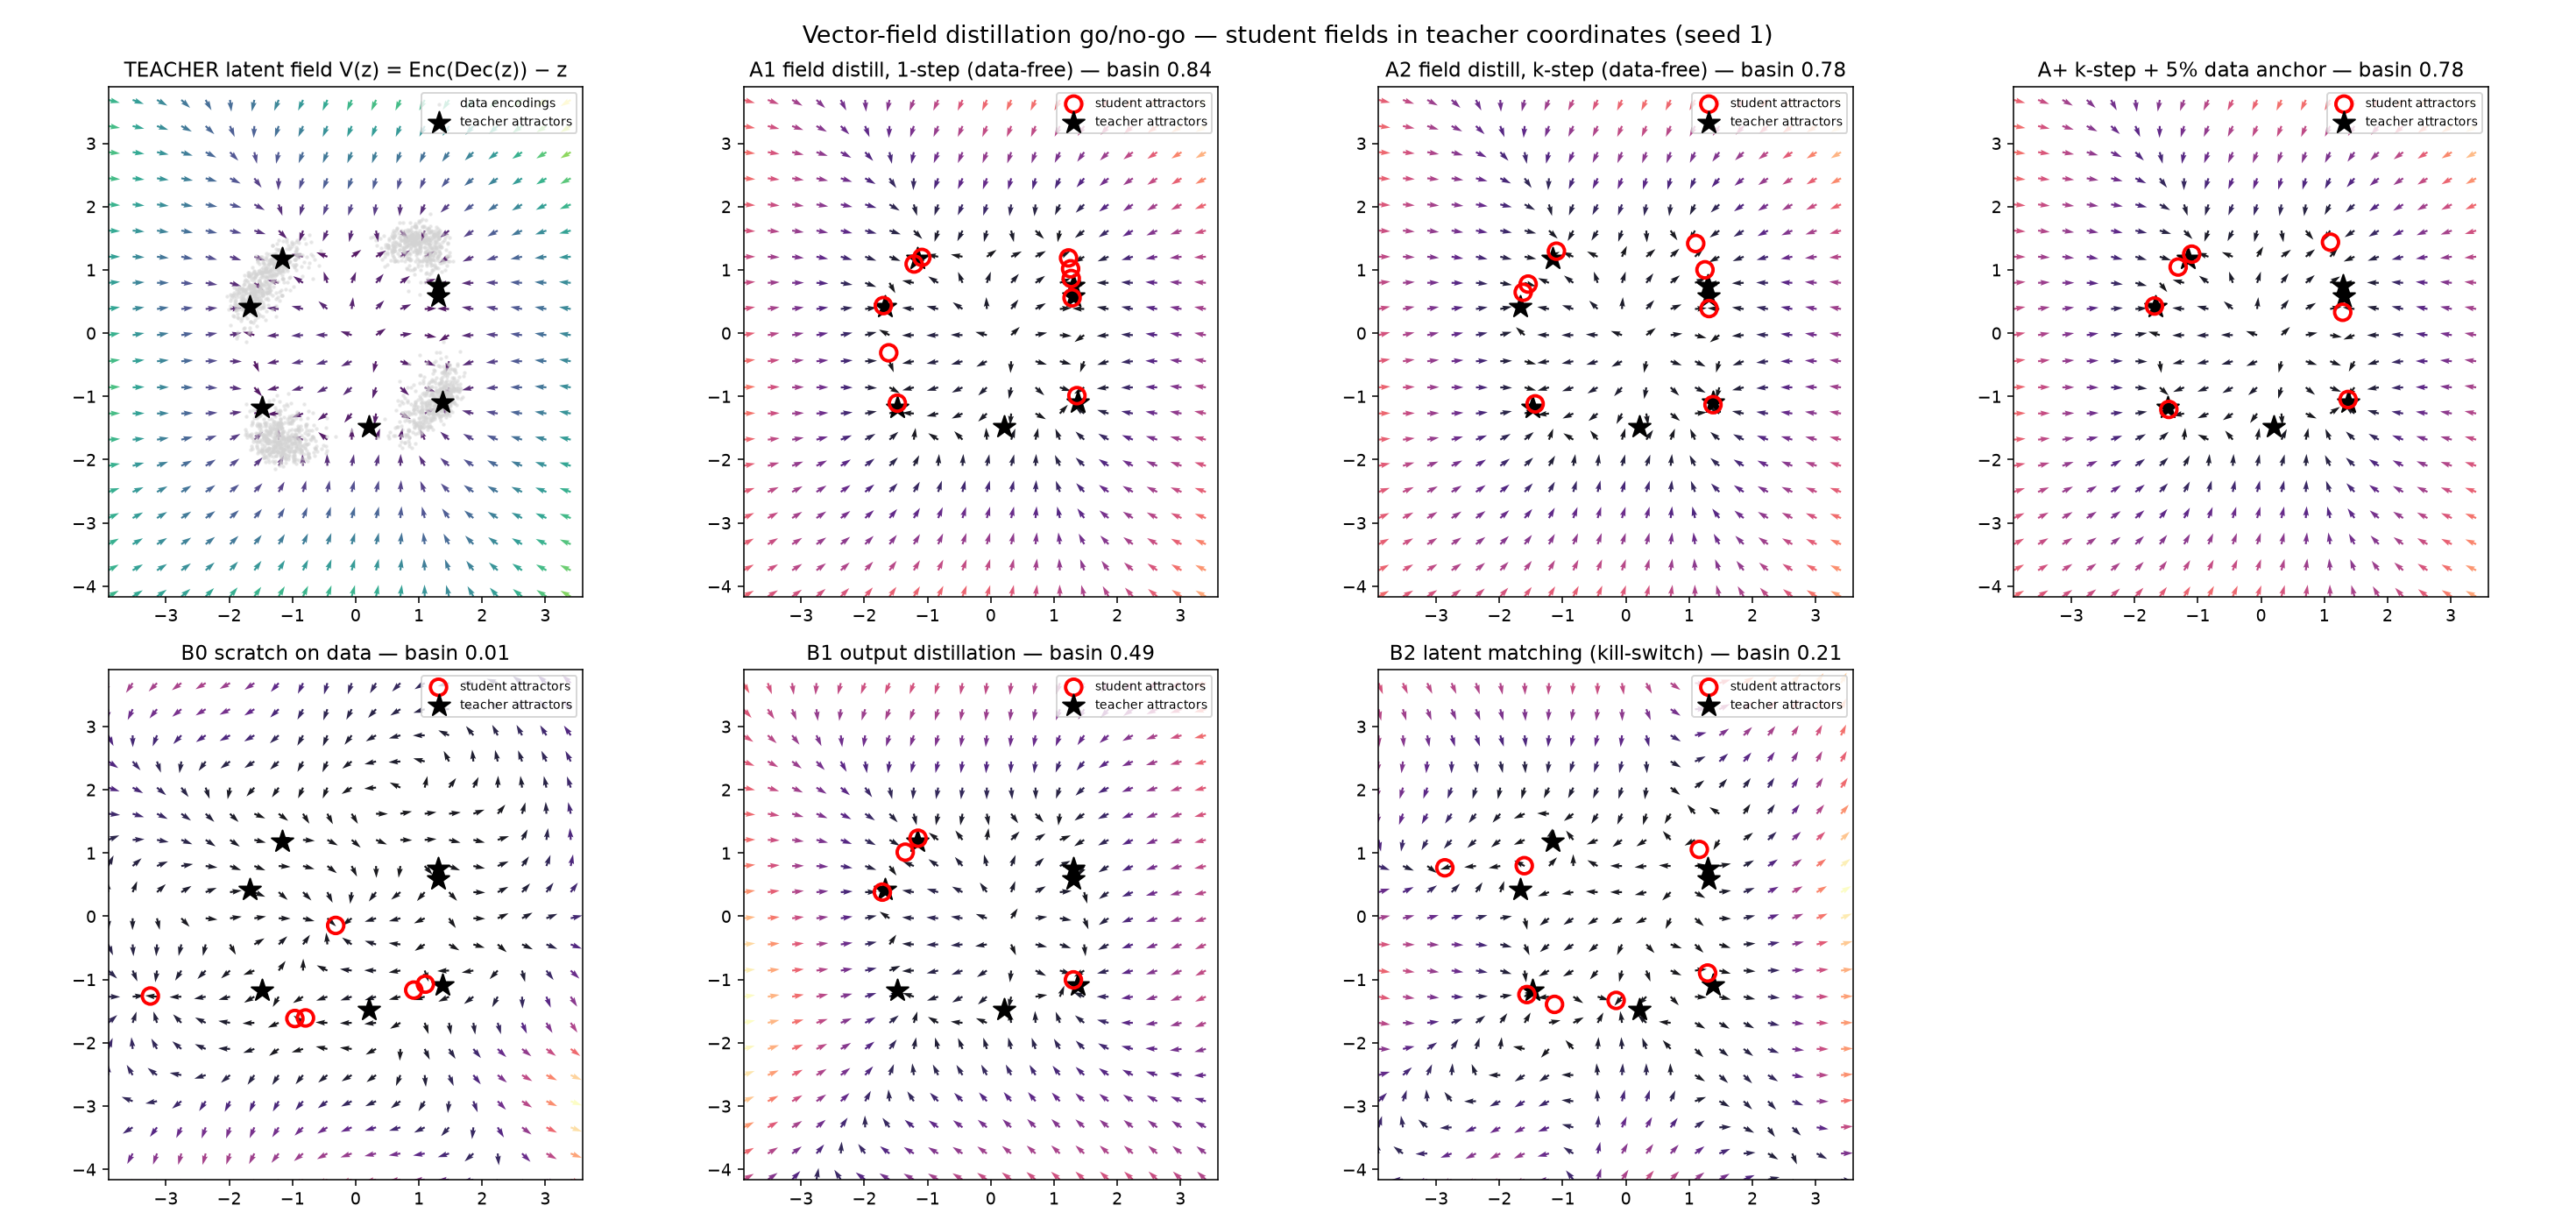
\includegraphics[width=\linewidth]{figures/field_panels.png}
  \caption{\textbf{Four ways to copy a network.} Each panel overlays a copy's terrain on the teacher's valleys (black stars; red circles are the copy's valleys). Field-matched copies reproduce the terrain. The network retrained from scratch on the same data builds unrelated terrain. Output distillation recovers part; feature matching almost none.}
  \label{fig:panels}
\end{figure}

\begin{plainterms}
Two students can read the same textbooks and organize the material differently. The scratch baseline is that second student: same data, unrelated terrain, agreement $0.00$. Copying the terrain is the only channel that reproduces how this particular network computes; methods that imitate its answers recover at most half.
\end{plainterms}

Longer supervision horizons do not help; per-step precision does. Multi-step and trajectory variants lost to the one-step objective in every test ($0.72$ vs $0.86$ contractive; $0.13$ vs $0.26$ memorizing; worse again on MNIST).

The teacher's training regime decides whether it can be copied, and the transition shows in reliability, not the mean. Sweeping denoising $\sigma$ from $0$ to $0.2$, the teacher's convergence fraction jumps from $0.71$ to $1.00$ between $\sigma = 0.045$ and $0.05$. At that level the seed spread of copyability collapses: seeds span $0.09$--$0.75$ below the transition and read $0.690$, $0.685$, $0.685$ at it. Transmission becomes deterministic when the source's field becomes fully convergent.

The same data falsify a stronger hypothesis. If copyability tracked model quality, it would peak with off-manifold robustness ($\sigma \approx 0.08$--$0.10$); instead, robustness degrades at $\sigma = 0.2$ while copyability rises to $0.99$. Copyability measures dynamical order, nothing else.

\section{The Wrong Observable and the Right One}

\begin{figure}[t]
  \centering
  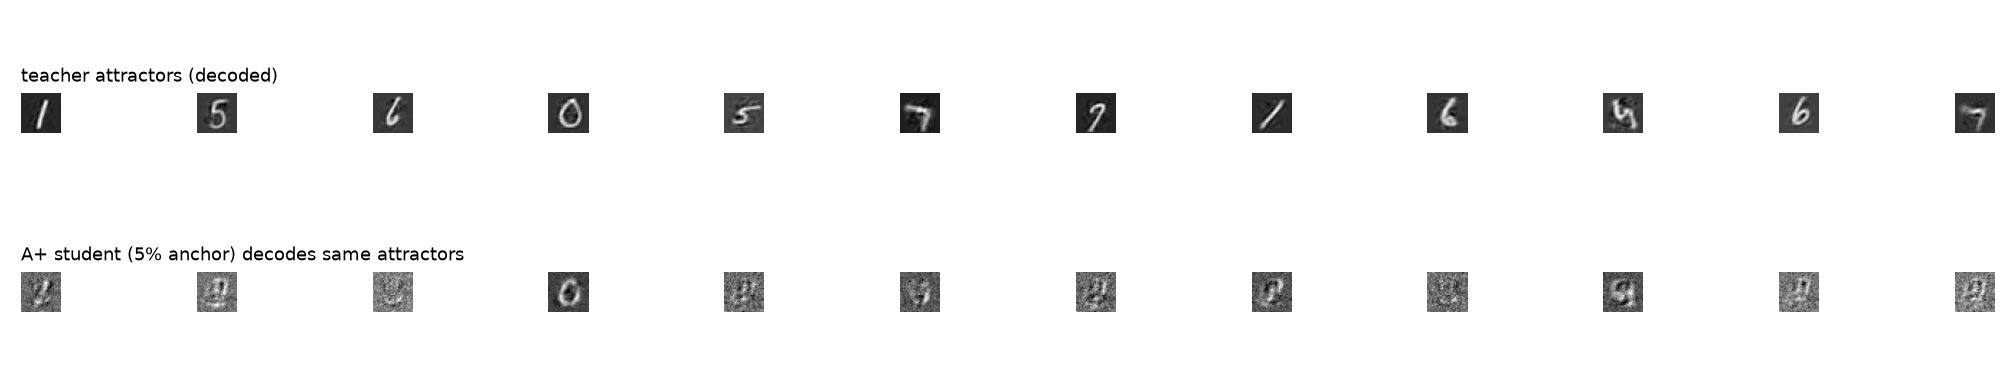
\includegraphics[width=\linewidth]{figures/mnist_attractors.png}
  \caption{\textbf{The valleys are memories.} On handwritten digits, the bottoms of the teacher's valleys, decoded to images, are crisp digit prototypes (top row). A copied student places its valleys at the same locations (bottom row: the same latent points through the student's decoder, blurry because the copy was only lightly anchored to image space).}
  \label{fig:mnist}
\end{figure}

\begin{plainterms}
On real images the valleys are concrete: each one is a remembered digit (Figure~\ref{fig:mnist}). The next result is about maps. A map that is slightly wrong everywhere but correct about which side of every ridge you are on will get you home. A map that is precise on average but wrong at the passes will not. Average error rewards the second map; the data below show it is the wrong measure of a copy.
\end{plainterms}

Mean field error, the quantity every regression minimizes, anti-correlates with basin transfer. On the same MNIST field, the parametric student attains NMSE $0.049$ and basin agreement $0.090$; a $10^6$-pair lookup table attains NMSE $0.397$ (eight times worse) and basin agreement $0.410$ ($4.6$ times better). A Gaussian-process carrier \citep{hoffman1991,rasmussen2006} tuned by held-out NMSE reaches basin agreement $0.000$--$0.004$; tuned by cosine preservation, it transfers partially. Basins are decided by where the displacement points near boundaries, not by its average size.

With the observable corrected, the high-dimensional wall separates into a budget and a ceiling. Parametric students fail MNIST at basin level (best $0.19$ against a $0.71$ ceiling), but the lookup carrier climbs $0.04 \to 0.28 \to 0.41$ across $16\mathrm{k} \to 262\mathrm{k} \to 10^6$ pairs with no plateau. The wall is sample budget, not dimension. The ceiling is the teacher's own boundary geometry: $\alpha = 0.454$ implies boundaries of dimension $\approx 15.5$ in a 16-dimensional latent space, nearly space-filling despite a convergence fraction of $0.97$, and it predicts the ceiling, $1 - f(\varepsilon_{\mathrm{probe}}) = 0.69$ against the measured $0.711$. Convergence fraction does not certify copyability; the flip-rate curve does.

\begin{plainterms}
The ceiling exists because boundaries can be crinkled like a coastline: zoom in and there is more crinkle. Near such a boundary a tiny nudge changes which valley the marble reaches, so even the teacher disagrees with itself between nearly identical starts. No copy can repeat a decision the original cannot repeat. The exponent $\alpha$ measures the crinkle, and with it the best any copy can do, before copying is attempted.
\end{plainterms}

The remaining parametric problem is reliability, not capacity. A student supervised by a $16{,}384$-pair GP reconstruction instead of the teacher is bimodal over six seeds ($0.008$, $0.387$, $0.004$, $0.309$, $0.496$, $0.004$). The best seed beats the $10^6$-pair lookup with $61\times$ fewer teacher queries. The failures are invisible in field space: all six seeds sit at cosine $0.82$--$0.83$, and only basin agreement separates them. The wrong-observable effect recurs at the supervision signal itself.

\section{Composition and Inheritance: Loss and Selection Are in the Carrier}

\begin{figure}[t]
  \centering
  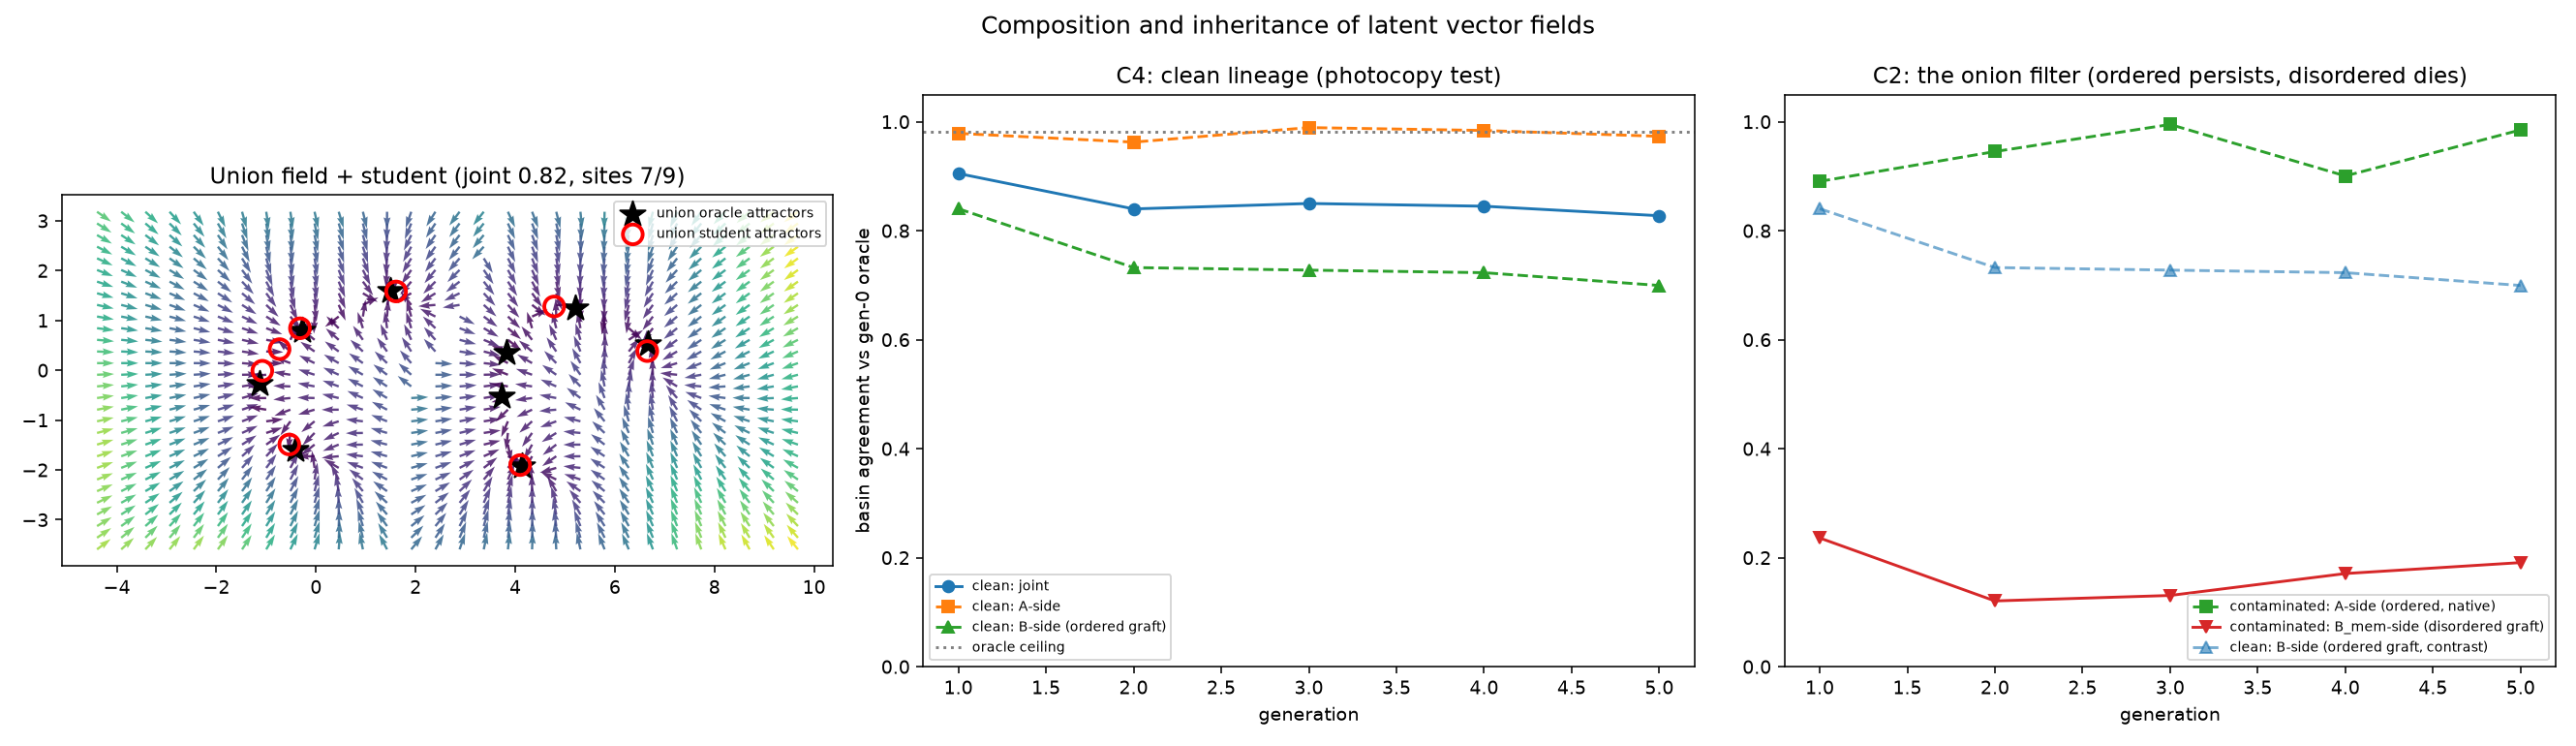
\includegraphics[width=\linewidth]{figures/gi.png}
  \caption{\textbf{Merging and inheriting knowledge.} Left: two specialist networks' terrains placed side by side in one designed frame, and a single data-free student whose valleys (red) land on both specialists' valleys (black). One network now holds what two knew. Center: five generations of copy-of-a-copy; the curves stay flat. Right: the filter. Ordered knowledge (green, blue) persists for five generations; a memorized, disordered graft (red) never enters the lineage.}
  \label{fig:gi}
\end{figure}

Fields from disjoint teachers union into one student, but only in a designed frame. The isometric union student holds both knowledge sets at joint agreement $0.82$ over five seeds (ceiling $0.98$), recovering up to 8 of 9 oracle attractor sites; no ancestor saw more than half the world (Figure~\ref{fig:gi}, left). Merged output distillation, given pooled data the union student never sees, scores $0.13$ with the grafted side at exactly $0.00$: behavioral cloning has no mechanism for placing disjoint knowledge. The input-consistent alternative, grafting $B$ where $A$'s encoder places $B$'s inputs, destroys the same knowledge (grafted side $0.14$). It compresses margins $3.6\times$ while leaving $\alpha$ essentially intact ($0.924$ vs $0.980$): a prefactor pathology, invisible to the exponent.

The composed knowledge is heritable, and inheritance failures come from the carrier, not the channel. Five generations of data-free re-distillation retain $91\%$ of joint agreement ($0.91 \to 0.83$) with stable attractor structure. A memorization-regime graft never enters the SGD lineage ($\leq 0.24$ throughout) while ordered structure persists beside it at $0.89$--$1.00$. Replacing the SGD student with a read-only $512^2$ lattice, with no optimization anywhere, removes every loss: the union sits at $0.99$ (ceiling $0.97$), the lineage is flat, and the memorized graft transmits at $0.68$, flat, $19/22$ sites. The field channel is nearly lossless and unselective. Loss and selection live in the lossy parametric carrier at fixed budget, so selection is a design parameter: the carrier budget determines what transmits.

\begin{plainterms}
Two specialists, each knowing half the world, are merged into a single student that has seen neither teacher's data, and it holds both bodies of knowledge (Figure~\ref{fig:gi}). The student then teaches a student, five times over, and the knowledge survives essentially intact. The lineage also filters: well-organized knowledge passes from generation to generation; rote memorization does not. The filter is not the copying process, since a perfect recording passes everything, memorization included. The filter is the finite capacity of the student. Knowledge forced through a small vessel keeps only what is general.
\end{plainterms}

\section{The Diagnostic at Ground Truth}

Tested where everything is exact, the $\alpha$ diagnostic keeps its ordering claims everywhere and its quantitative claims only in their measured scope. On Newton fractals ($n = 2..5$), $\alpha$ matches independently box-counted boundary dimension within $0.07$, orders student basin agreement at Spearman $+1.0$, and computes it: the pricing law $\mathrm{basin} = 1 - f(\delta_{\mathrm{eff}})$ predicts all twelve students within $0.01$--$0.03$. On the magnetic pendulum, $\alpha$ tracks the physical damping dial, matches box counts within $0.14$, and orders again at $+1.0$. The pricing law degrades off the contracting regime (median gap $0.187$): ordering travels unconditionally, pricing does not. The pendulum also supplies the law behind the reliability transition: seed spread at fixed budget anti-correlates with $\alpha$ at Spearman $-1.0$. One pre-registered gate failed, informatively: at fixed optimization budget, more pairs made parametric students worse ($0.879 \to 0.640$). Lookup carriers scale with pairs alone; parametric students need sample and optimization budgets scaled together.

Boundary geometry is generated, not stored. Newton students reproduce their teacher's $\alpha$ within $0.02$--$0.03$. The student learns the smooth one-step map, and the fractal boundary re-emerges under iteration, the basin-boundary counterpart of attractor climate replication in reservoir computing \citep{pathak2017,rohm2021,hart2024}. Finite capacity never pays for representing the boundary; copy error costs only where it meets the boundary.

Iterated copying obeys a law that single copies do not. Across seven single teacher-to-student pairs there is no systematic smoothing. Down a five-generation lineage, $\alpha$ climbs $0.765 \to 1.112$ while self-consistency rises $0.972 \to 0.993$ and fidelity to the origin falls $0.828 \to 0.520$. Copies of copies grow more definite and less faithful. Self-agreement is therefore not evidence of fidelity: the MNIST student pairs a self-ceiling of $0.799$, above its teacher's $0.711$, with basin agreement $0.055$. The corrected instrument is the full $f(\varepsilon)$ curve at the copy's error scale; the bare exponent is scale-blind.

\begin{plainterms}
A story retold down a chain of narrators gets smoother with each telling and drifts from what happened. Model lineages do the same, measurably: each generation's decision boundaries are smoother and more confident, and each is further from the original. Confidence is usually the only thing an outside observer checks. A fifth-generation copy looks more decisive than the original while agreeing with it about half the time.
\end{plainterms}

\section{Scope}

All positive basin-level results are 2-D latent, laptop scale, two to five student seeds, one teacher seed per condition, affine-only alignment. At 16 dimensions, parametric carriers remain unreliable while read-out carriers cross the wall at budget. GP reconstruction efficiency is teacher-dependent ($0.48$ at 16k pairs on a retrained teacher; $0.095 \pm 0.060$ on the original) and remains open. Nothing here concerns capability gain: a union student knows the union of its ancestors' knowledge and nothing more.

\section{Conclusion: Toward a True Knowledge Benchmark}

The instruments validated above generalize beyond autoencoders: they apply to any model whose dynamics sort initial conditions into outcomes. A true knowledge benchmark asks not whether a model matches outcomes at one setting, but whether its own dynamics sort initial conditions into the same futures as reality, with the same sharpness, at the same perturbation scales.

The Basin-of-Attraction Benchmark (scoped July 12, 2026, companion project) applies these instruments to video world models, whose predictor, the actual world model, has no dynamical evaluation anywhere in the literature. It has three scores, with all perturbations in world space: physical units, never latent, which removes the metric-choice problem and makes the benchmark architecture-agnostic.

\begin{itemize}\setlength{\itemsep}{0.6em}
  \item \textbf{Basin agreement} $A$: the fraction of probe initial conditions whose settled outcome matches the simulator's.
  \item \textbf{Decidability calibration} $\Omega$: the model's flip-rate curve against reality's, summarized by the overconfidence index $\Omega = \int (f_{\mathrm{true}} - f_{\mathrm{model}})\, d(\log \varepsilon)$. A positive $\Omega$ means the model's boundary is smoother than reality's: confident but wrong near decisions, the failure mode the lineage law produces and no static probe detects.
  \item \textbf{Attractor census} $C$: collapse detection at the dynamics level.
\end{itemize}

The design keystone comes from the ground-truth study: every scenario family carries a roughness dial that moves the true $\alpha$, so the benchmark tests whether a model tracks reality's decidability.

The methodology carries over: pre-registered gates, context-only controls published next to every score, full curves rather than bare exponents, no pricing claims outside contracting regimes, ill-defined outcomes reported rather than scored.

The same machinery ports to systems whose fields are trained rather than emergent \citep{ho2020ddpm,song2021score} and to recurrent-depth models whose step displacements are already measured \citep{pappone2025}. Beyond world models, the instruments define the language-model test of the order law: the full flip-rate curve per capability, empirically calibrated perturbation scales, ratchet effects expected only under repeated re-distillation. The endpoint is a single audit: given any model, measure $f(\varepsilon)$ on its decision boundaries and know, before any transfer, merge, or distillation is attempted, what it can teach, what it can inherit, and what it will lose.

\subsection*{Reproducibility}

All experiments were implemented in MLX and run on a single Apple laptop. The released harness contains one module per experiment with fixed seeds, JSON run records for every number reported, and the scripts that generate every figure: \url{https://github.com/Veso-AI-Open-Source/knowledge-as-dynamics}.

\begin{thebibliography}{99}

\bibitem[Fumero et al.(2025)]{fumero2025}
M.~Fumero, L.~Moschella, E.~Rodol\`a, and F.~Locatello.
\newblock Navigating the latent space dynamics of neural models.
\newblock \emph{arXiv preprint arXiv:2505.22785}, 2025.

\bibitem[Grebogi et al.(1983)]{grebogi1983}
C.~Grebogi, S.~W. McDonald, E.~Ott, and J.~A. Yorke.
\newblock Final state sensitivity: An obstruction to predictability.
\newblock \emph{Physics Letters A}, 99(9):415--418, 1983.

\bibitem[Hart(2024)]{hart2024}
J.~D. Hart.
\newblock Attractor reconstruction with reservoir computers: The effect of the reservoir's conditional Lyapunov exponents on faithful attractor reconstruction.
\newblock \emph{Chaos}, 34(4):043123, 2024.

\bibitem[Hinton et al.(2015)]{hinton2015}
G.~Hinton, O.~Vinyals, and J.~Dean.
\newblock Distilling the knowledge in a neural network.
\newblock \emph{arXiv preprint arXiv:1503.02531}, 2015.

\bibitem[Ho et al.(2020)]{ho2020ddpm}
J.~Ho, A.~Jain, and P.~Abbeel.
\newblock Denoising diffusion probabilistic models.
\newblock In \emph{Advances in Neural Information Processing Systems}, 2020.

\bibitem[Hoffman and Ribak(1991)]{hoffman1991}
Y.~Hoffman and E.~Ribak.
\newblock Constrained realizations of Gaussian fields: A simple algorithm.
\newblock \emph{The Astrophysical Journal}, 380:L5--L8, 1991.

\bibitem[McDonald et al.(1985)]{mcdonald1985}
S.~W. McDonald, C.~Grebogi, E.~Ott, and J.~A. Yorke.
\newblock Fractal basin boundaries.
\newblock \emph{Physica D}, 17(2):125--153, 1985.

\bibitem[MEDAL(2026)]{medal2026}
MEDAL: Manifold embedding distillation via autoencoder learning.
\newblock \emph{arXiv preprint arXiv:2605.24244}, 2026.

\bibitem[Distilling Latent Manifolds(2026)]{latentmanifolds2026}
Distilling latent manifolds: Resolution extrapolation by variational autoencoders.
\newblock \emph{arXiv preprint arXiv:2603.14536}, 2026.

\bibitem[Pappone et al.(2025)]{pappone2025}
F.~Pappone, D.~Crisostomi, and E.~Rodol\`a.
\newblock Two-scale latent dynamics for recurrent-depth transformers.
\newblock \emph{arXiv preprint arXiv:2509.23314}, 2025.

\bibitem[Park et al.(2019)]{park2019rkd}
W.~Park, D.~Kim, Y.~Lu, and M.~Cho.
\newblock Relational knowledge distillation.
\newblock In \emph{IEEE/CVF Conference on Computer Vision and Pattern Recognition}, 2019.

\bibitem[Pathak et al.(2017)]{pathak2017}
J.~Pathak, Z.~Lu, B.~R. Hunt, M.~Girvan, and E.~Ott.
\newblock Using machine learning to replicate chaotic attractors and calculate Lyapunov exponents from data.
\newblock \emph{Chaos}, 27(12):121102, 2017.

\bibitem[Rasmussen and Williams(2006)]{rasmussen2006}
C.~E. Rasmussen and C.~K.~I. Williams.
\newblock \emph{Gaussian Processes for Machine Learning}.
\newblock MIT Press, 2006.

\bibitem[R\"ohm et al.(2021)]{rohm2021}
A.~R\"ohm, D.~J. Gauthier, and I.~Fischer.
\newblock Model-free inference of unseen attractors: Reconstructing phase space features from a single noisy trajectory using reservoir computing.
\newblock \emph{Chaos}, 31(10):103127, 2021.

\bibitem[Romero et al.(2015)]{romero2015fitnets}
A.~Romero, N.~Ballas, S.~E. Kahou, A.~Chassang, C.~Gatta, and Y.~Bengio.
\newblock FitNets: Hints for thin deep nets.
\newblock In \emph{International Conference on Learning Representations}, 2015.

\bibitem[Song et al.(2021)]{song2021score}
Y.~Song, J.~Sohl-Dickstein, D.~P. Kingma, A.~Kumar, S.~Ermon, and B.~Poole.
\newblock Score-based generative modeling through stochastic differential equations.
\newblock In \emph{International Conference on Learning Representations}, 2021.

\bibitem[Srinivas and Fleuret(2018)]{srinivas2018jacobian}
S.~Srinivas and F.~Fleuret.
\newblock Knowledge transfer with Jacobian matching.
\newblock In \emph{International Conference on Machine Learning}, 2018.

\bibitem[Tian et al.(2020)]{tian2020crd}
Y.~Tian, D.~Krishnan, and P.~Isola.
\newblock Contrastive representation distillation.
\newblock In \emph{International Conference on Learning Representations}, 2020.

\bibitem[Tung and Mori(2019)]{tung2019similarity}
F.~Tung and G.~Mori.
\newblock Similarity-preserving knowledge distillation.
\newblock In \emph{IEEE/CVF International Conference on Computer Vision}, 2019.

\end{thebibliography}

\end{document}
